% Chapter Template

% Main chapter title
%\chapter[toc version]{doc version}
\chapter{System Architecture \& Design}

% Short version of the title for the header
%\chaptermark{version for header}

% Chapter Label
% For referencing this chapter elsewhere, use \ref{ChapterTemplate}
\label{Chapter4SystemArchitectureDesign}

% Write text in here
% Use \subsection and \subsubsection to organize text

Delivering reliable, scalable automated assessment of virtualized networks requires a system built on solid principles of 
virtualization and automation. This chapter outlines the architecture of the proposed system, detailing the key components 
and how they interact to enable evaluation of student-submitted network exercises.

The system is designed to provide each student with a working environment where custom virtual network topologies can be 
deployed, configured, and tested. To achieve this, the platform integrates several technologies—such as\ac{gns3} for network 
emulation,\ac{pve} for virtualization, and Nornir for configuration testing—alongside an asynchronous web-based\ac{api} layer for 
user interaction and system communications.

This section provides a high-level overview of the system, the rationale behind its design choices, and the fundamental 
components that make up its architecture.

\section{Functional Use Cases}

\section{System Architecture Overview}
    The architecture is divided into several key components, each responsible for a specific aspect of the system's functionality. 
    The main components of the system architecture are as follows:

    \begin{itemize}
        \item \textbf{Web Application:} The web application serves as the main interface for users to interact with the system. It provides 
        endpoints for, amongst others, evaluation, creation  and viewing available exercises. The application is designed to be asynchronous 
        where possible, allowing for efficient handling of multiple requests simultaneously.
        
        \item \textbf{Proxmox VE:}\ac{pve} is responsible for creating and managing\ac{vm}s that host the network devices used in 
        the exercises. This component interacts with the web application and all communication is done asynchronously through 
        the\ac{pve}\ac{rest}\ac{api}, which allows for efficient communication, keeping the web application responsive, while also 
        keeping the components decoupled.
        
        \item \textbf{GNS3:}\ac{gns3} is used to emulate all the components of the virtual networks to be configured by students, 
        using various types of virtualization detailed earlier. Communication with\ac{gns3} is done through 
        the\ac{gns3}\ac{rest}\ac{api} by the web application during template\ac{vm} creation and validation

        \item \textbf{Nornir:} This automation framework is used for validating device configurations. It connects to the 
        virtualized devices, executes commands, and compares the output to expected results to determine correctness.
        Currently this component is integrated into the web application
    \end{itemize}

\section{Proxmox VE}

    \ac{pve} functions as the virtualization backbone of the system, enabling the creation and management of Linux-based\ac{vm}s 
    which in turn host services for use by students. Each\ac{vm} runs a lightweight Linux-based operating system with a 
    dedicated\ac{gns3} instance, providing a self-contained environment for deploying and configuring virtual networks 
    and their components.

    All\ac{pve}-related operations—such as cloning, starting, templating, and deletion—are fully automated and triggered by the 
    web application. Under normal operation ,after doing pre-required setup, no further manual intervention using the\ac{pve} web 
    UI or shell utilities is required; such intervention is only necessary when the system's error handling mechanisms detect failures 
    that cannot be automatically resolved. To securely execute these operations, the application authenticates to the\ac{pve}\ac{api} 
    using token-based authentication. The required credentials and configuration parameters are securely injected via environment variables\unsure{this may change}, 
    while the time limited token is stored in memory, ensuring that only authorized and properly configured processes can interact 
    with the\ac{pve} infrastructure.

    \subsection{Why Proxmox VE?}

        \ac{pve} was chosen for several compelling reasons that make it ideal for it to be choosen as our virtualization platform. First, 
        it's completely free to use for all core functionality, with no hidden costs or licensing traps. Unlike proprietary solutions that 
        charge per CPU core or socket,\ac{pve} lets us scale up our infrastructure without worrying about surprise licensing fees.

        The platform's support for both containers and\ac{vm}s within a single management interface gives us tremendous flexibility. We 
        can run lightweight\ac{lxc} for applications that dont require a full\ac{vm} while using full\ac{vm}s where required seamlessly. 
        This hybrid approach would not be as straightforward with other solutions, like VMware ESXi.

        We also value storage system's flexibility with LVM-thin provisioning allows efficient snapshotting of student environments while 
        maintaining good performance.

        Looking ahead,\ac{pve}'s built-in support for emerging technologies like software-defined networking and its robust role-based 
        access control system means our project still has room to grow into\ac{pve}. The active open-source development community ensures 
        continuous improvements without vendor lock-in.

    \subsection{Proxmox VE Limitations}

        During development, we encountered several challenges when interfacing programmatically with\ac{pve}. One of th most significant 
        issues stemmed from the platform's limited visibility into non-instantaneous operations - particularly for tasks like\ac{vm} cloning, 
        where the system did not provide task ids in the\ac{http} responses. This forced us to implement custom polling mechanisms to reliably 
        determine operation completion states where possible.

        A more critical limitation emerged in\ac{pve}ac{rest}ac{api}'s resilience characteristics. During stress testing, we discovered that 
        even moderate request volumes done using a single machine running sequential code could overwhelm the single-node cluster's management 
        daemon, triggering frequent\ac{http} 500 errors. These reliability constraints necessitated the development of protective measures 
        including exponential backoff retry logic and strict client-side concurrent request limiting to maintain system stability.

    \subsection{Proxmox VE Firewall}

        \ac{pve} comes bundled with a iptables-based firewall implementation that can be enabled and configured at different levels.

        The Proxmox host-level firewall provides essential features for securing student work environments, during examination 
        periods, preventing student machines and the virtualized network equipments in them from communicating with outside networks.

        This is done by adding firewall rules at the host level, meaning to each relevant student\ac{vm}, that disable communications
        in both directions, with the exception of the machine that is responsible for configuration validation.

        By default this behavior is not active and must be enabled on an as-needed basis, typically when a controlled assessment 
        environment is required for more rigorous situations such as examinations.

        In future iterations it may also be valuable to develop this further and making this feature less rigid as it may be interesting 
        to have exercises that communicate with devices on the internet.
    
    \subsection{Exploration of containers as a full substitute for VMs}

        During development, we attempted to minimize\ac{vm} usage where possible to accommodate as much scaling potencial as possible. 
        The introduction of the\ac{gns3} web interface allowed the machines hosting\ac{gns3} instances to operate in a headless manner, 
        removing the need for direct student interaction with the host machine. This eliminated desktop environment requirements and 
        significantly reduced memory overhead, improving scalability.

        We further explored replacing\ac{vm}s entirely with containers, which promised additional resource savings. However, this approach 
        proved unworkable due to fundamental technical constraints. Effective emulation requires\ac{kvm} acceleration, which presents 
        two problematic scenarios in containerized environments: either running unprivileged containers without\ac{kvm} access (resulting 
        in unacceptable performance degradation) or configuring privileged containers or containers with\ac{kvm} passthrough (introducing 
        serious security vulnerabilities).

        Given that software emulation without\ac{kvm} acceleration delivers poor performance for interactive use, we abandoned containerization 
        as a complete\ac{vm} replacement. The\ac{vm}-based architecture remains necessary to maintain both performance through hardware 
        acceleration and proper isolation between student environments.

        \subsubsection{VM Lifecycle}

            The lifecycle of a\ac{vm} begins when a new exercise is created by a priviledged user through the web application. 
            Upon exercise creation, the platform automatically clones a pre-configured base template\ac{vm} stored in\ac{pve}. This new instance 
            undergoes a configuration process where the provided\ac{gns3} project file is imported and a series of user-defined commands are executed 
            across the provided network topology. Once the setup is finalized, the configured\ac{vm} is converted into a new template\ac{vm} that 
            is tailored to that exercise.

            When students are enrolled in an exercise, the system generates individual work environments, by creating linked clones from these 
            exercise-specific templates. Each student receives their own isolated\ac{vm} instance that precisely mirrors the original template's 
            configuration. This cloning approach ensures both consistency across student environments and rapid provisioning, as linked clones 
            avoid the overhead of full disk copies while maintaining the template's baseline configuration. The use of linked clones significantly 
            reduces both storage requirements and deployment time compared to traditional full cloning methods.
        
\section{GNS3}

    \ac{gns3} serves as the core network virtualization component in our system, providing the capability to emulate various network devices 
    and topologies. The platform was selected for several key advantages: its remote web-based interaction, the intuitive drag-and-drop interface 
    simplifies usage, and its broad device support accommodates both terminal-based and GUI network equipment and full computers. Additionally, 
    \ac{gns3}'s\ac{api} allows for programmatic interaction, which proves essential for automation within our environment.

    Currently, the system requires manual preparation of the base \ac{gns3} template\ac{vm}. During initial setup, an administrator must first create 
    and configure a new\ac{vm}, then proceed to install and set up the\ac{gns3} environment. The final preparation step involves importing all 
    necessary device images, including routers, switches, and other equipment that will be available for student exercises.

    This base template then serves as the source for all subsequent student instances through\ac{pve}'s cloning functionality. While this 
    manual setup process adds initial configuration overhead, it ensures complete control over the base environment and allows for careful 
    curation of the included device images.

    The system achieves scalability through multiple \ac{vm} instances running in \ac{pve}, each hosting an independent \ac{gns3} environment. 
    This architecture enables concurrent usage by multiple students on a single physical host. For future expansion, the design supports 
    horizontal scaling by adding additional nodes to the \ac{pve} cluster, allowing the platform to accommodate growing numbers of users 
    without requiring complete architectural changes.

    \begin{figure}
        \centering
          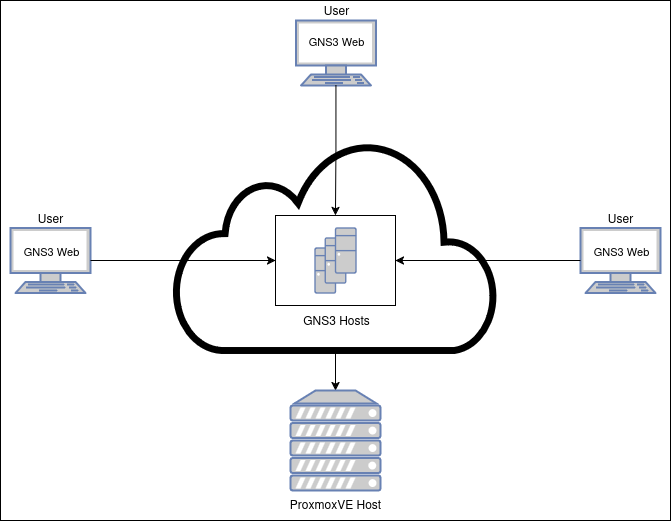
\includegraphics[width=.95\linewidth]
            {4SystemArchitectureDesign/user-gns3-proxmox-diagram.png}
        \caption{A diagram showcasing how users interact with the system's resources on a high level}
      \hfill
    \end{figure}

\section{High-level architecture}

    \subsection{Available Hardware }

        The current deployment hosts all internal system components (those shown in the architecture diagram excluding the external LDAP instance) 
        on a single physical server with the following specifications.

        \begin{table}[h]
            \centering
            \caption{System Hardware Specifications}
            \begin{tabular}{|l|l|}
                \hline
                \textbf{Component} & \textbf{Specification} \\ \hline
                Processor & Intel Core i7-9700K \\ \hline
                Memory & 32GB DDR4 @ 2666MHz \\ \hline
                Storage & 1TB Samsung 970 EVO Plus NVMe SSD \\ \hline
                Graphics & NVIDIA GTX 1650 \\ \hline
            \end{tabular}
        \end{table}

        This machine's specifications, while capable, create inherent memory constraints. With 32GB of available RAM, practical\ac{vm} allocation 
        becomes the primary bottleneck. For instance, when deploying\ac{gns3} instances each configured with 4GB of memory, the system can maintain 
        only seven active\ac{vm}s simultaneously. This limitation accounts for the\ac{pve} hypervisor's own memory overhead before encountering swap 
        usage, which would degrade performance.

    \subsection{User Interface}
        The system employs a dual-interface web architecture accessible through standard browsers. For administrative functions and exercise management, 
        users interact with Jinja2-rendered HTML pages delivered by the web application. These templates handle all developed features, like user 
        authentication,\ac{vm} interaction etc.

        When working on networking exercises, users can transition to the \ac{gns3}-web interface by clicking a button. This dedicated environment 
        provides direct access to the user's virtual network devices, as required by each exercise scenario. This integration ensures users experience 
        a cohesive workflow from exercise selection to practical implementation without needing multiple authentication steps or application switches.

    \subsection{Web Application}

        The web application serves as the primary interface through which users interact with the system. It is built using the FastAPI 
        framework, following a migration from an earlier prototype developed using Flask, and follows an asynchronous-first, modular 
        architecture that provides scalable interactions with other system components.

        The application exposes a\ac{rest}\ac{api} that supports endpoints for user authentication, exercise creation, virtual 
        machine management, and configuration validation. It acts as the coordinator for the entire system, triggering operations 
        in\ac{pve},\ac{gns3}, and Nornir based on user actions.

        Wherever possible, asynchronous I/O is employed to prevent blocking during operations such as\ac{api} calls to\ac{pve}.
        Multiprocessing is also utilized to handle configuration validation. This keeps the system responsive and performant, 
        especially when handling multiple simultaneous requests from different users.

        Internally, the application is designed to be stateless and maintain minimal runtime state.  Most essential information—such 
        as user accounts, defined exercises, and student-to-VM mappings—is persisted in a relational database rather than stored in 
        memory. Configuration values such as API tokens, base URLs, and database credentials are injected via environment variables 
        to decouple deployment-specific settings from the application code. This design improves reliability, supports concurrent 
        usage, and enables horizontal scalability if deployed across multiple instances. 

        To ensure maintainability and modularity, interactions with external services like\ac{pve} and\ac{gns3} are isolated in 
        dedicated modules. These serve as abstraction layers between the application logic and third-party\ac{api}s, exposing clean, 
        reusable interfaces while hiding low-level implementation details. For example,\ac{pve}-related operations such as\ac{vm} 
        creation and deletion are handled in a separate module (e.g services/proxmox.py), as are all\ac{gns3}-related tasks. This 
        separation of concerns improves the structure of the codebase and simplifies future maintainability by being more readable.

        To help with development and testing, the application automatically generates OpenAPI-compliant documentation, allowing 
        developers to explore and interact with available endpoints. This self-documenting behavior streamlines integration 
        testing and encourages a more agile development process.

        Finally, to safeguard user data and infrastructure control points, the application enforces secure authentication mechanisms 
        using\ac{jwt} ensuring that only authorized users can trigger actions on shared resources.

    \begin{figure}
        \centering
            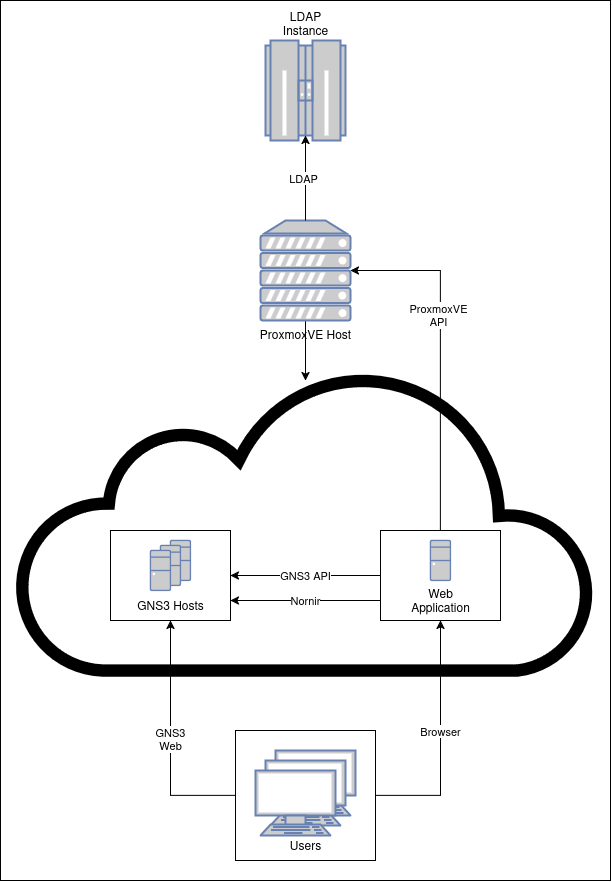
\includegraphics[width=.95\linewidth]
                {4SystemArchitectureDesign/system-diagram.png}
            \caption{A diagram showcasing a high level overview of the system's main components}
        \hfill
    \end{figure}

    \subsection{Virtualization Components}

        The system employs a hybrid virtualization approach using\ac{pve} as the foundational platform. The usage of containers was 
        explored but it was found unsuitable for our main use case of virtualization,\ac{gns3} instances. However there remains one valid 
        usage for containers for the project, which is hosting the web application. However this component may also be optionally hosted in 
        a separate physical machine.

        For network emulation, the system utilizes full\ac{kvm}-based virtual machines, each hosting a\ac{gns3} instance. These\ac{vm}s 
        provide the necessary hardware virtualization support for nested device emulation, particularly crucial for fast virtualization. 
        Finally, by the use of linked clones and storage-efficient backing filesystems, in this case LVM-thin, allows the system to rapidly 
        provision\ac{vm}s while minimizing storage usage.
    
    \subsection{Evluation component}

        The system employs a modular evaluation framework built on Nornir to validate configurations across virtualized network devices. 
        At its core, this component utilizes specialized Python classes called "modules" that encapsulate platform-specific validation logic. 
        Each module is responsible for three key functions: identifying the target device's platform (such as Cisco IOS, Linux, or VPCS), 
        executing the appropriate validation commands for that platform, and interpreting the command output using regular expressions to d
        etermine configuration correctness.

        The architecture follows an object-oriented design pattern with a base \texttt{CommandModule} class that handles common functionality. 
        This parent class manages the Nornir inventory initialization and provides essential methods like platform detection and command execution. 
        The actual validation logic is implemented in child classes that inherit from \texttt{CommandModule}, with each subclass specializing in 
        a particular type of network test. For example, the included \texttt{PingModule} implements platform-specific variants of the ping command 
        and corresponding response interpretation methods. This design promotes code reuse while allowing easy extension for new test types, as 
        developers can create additional modules by simply extending the base class and implementing the required platform-specific methods.
        
        Configuration validation occurs through a multi-stage process. When a test is initiated, the system first identifies the target device's 
        platform through Nornir's inventory system. It then dispatches the appropriate platform-specific command variant, such as the Cisco IOS-style 
        ping command for routers versus the Linux \texttt{ping -c} syntax for Linux hosts. The module captures and sanitizes the raw command output, 
        removing terminal control sequences and other artifacts before applying regular expressions to assess the results. For connectivity tests like 
        ping, the interpretation logic calculates success rates against a configurable tolerance threshold defined in the system constants.
        
        The evaluation framework supports several advanced features to enhance reliability and debugging. Command timeouts are managed to prevent 
        hanging operations, with a default window that can be tuned as needed. Future extensions could incorporate snapshot functionality, allowing 
        the system to capture and compare device states at different points during an exercise, though this capability is not currently implemented 
        in the base version. The modular architecture ensures such enhancements can be added without disrupting existing validation workflows.

    \subsection{Storage component}
        
        The system has two main components regarding storage, one for the database needs of the web application and one for the disks of the \ac{vm}s.

        \subsubsection{Virtual machine storage}

            For virtual machine storage, the system utilizes LVM-thin provisioning to optimize disk space utilization across student environments. 
            This storage backend enables efficient cloning operations through copy-on-write semantics while supporting advanced features like snapshot 
            preservation. LVM-thin's space-efficient cloning creates a robust foundation for the system's data needs.

        \subsubsection{Web application database}

            The SQLite database serves as the central repository for all application data, leveraging SQLModel as an ORM layer that combines Pydantic 
            validation with SQLAlchemy's database capabilities. This hybrid approach provides both runtime type safety and efficient database operations, 
            while Alembic handles schema migrations to accommodate evolving data requirements.

            The database schema organizes information across several interrelated models. User management builds upon a base \texttt{CustomBase} class 
            that automatically tracks creation timestamps, with the \texttt{User} model storing authentication credentials, administrative privileges, 
            and relationships to both submissions and virtual machine instances. The \texttt{Exercise} model captures lab configuration details, including 
            \ac{json}-serialized validation rules and device configurations stored as text fields due to SQLite's native type limitations.\ac{vm} 
            provisioning is managed through the \texttt{TemplateVm} and \texttt{WorkVm} hierarchy, where template instances maintain the base\ac{gns3} 
            project configurations and spawned work environments link back to both users and exercises. The \texttt{Submission} model completes the 
            core data structure by tracking student attempts, scores, and evaluation outputs while maintaining referential integrity through SQLAlchemy relationships.